\chapter{Introduction}
\label{sec:intro}

\iffale
This thesis is financed by BORDER 6, a interdomain \acf{TE} solution provider for stub \acf{AS}. 
It features a platform enabling performance oriented interdomain TE through continuous measurements.
Upon its request, we study in this thesis the various problems encountered in making better use of these available measurements to improve the TE platform from multiple aspects: scalability, measurement interpretation and performance visibility.
\fi

\section{Intradomain Routing}
\begin{figure}[!htb]
\centering
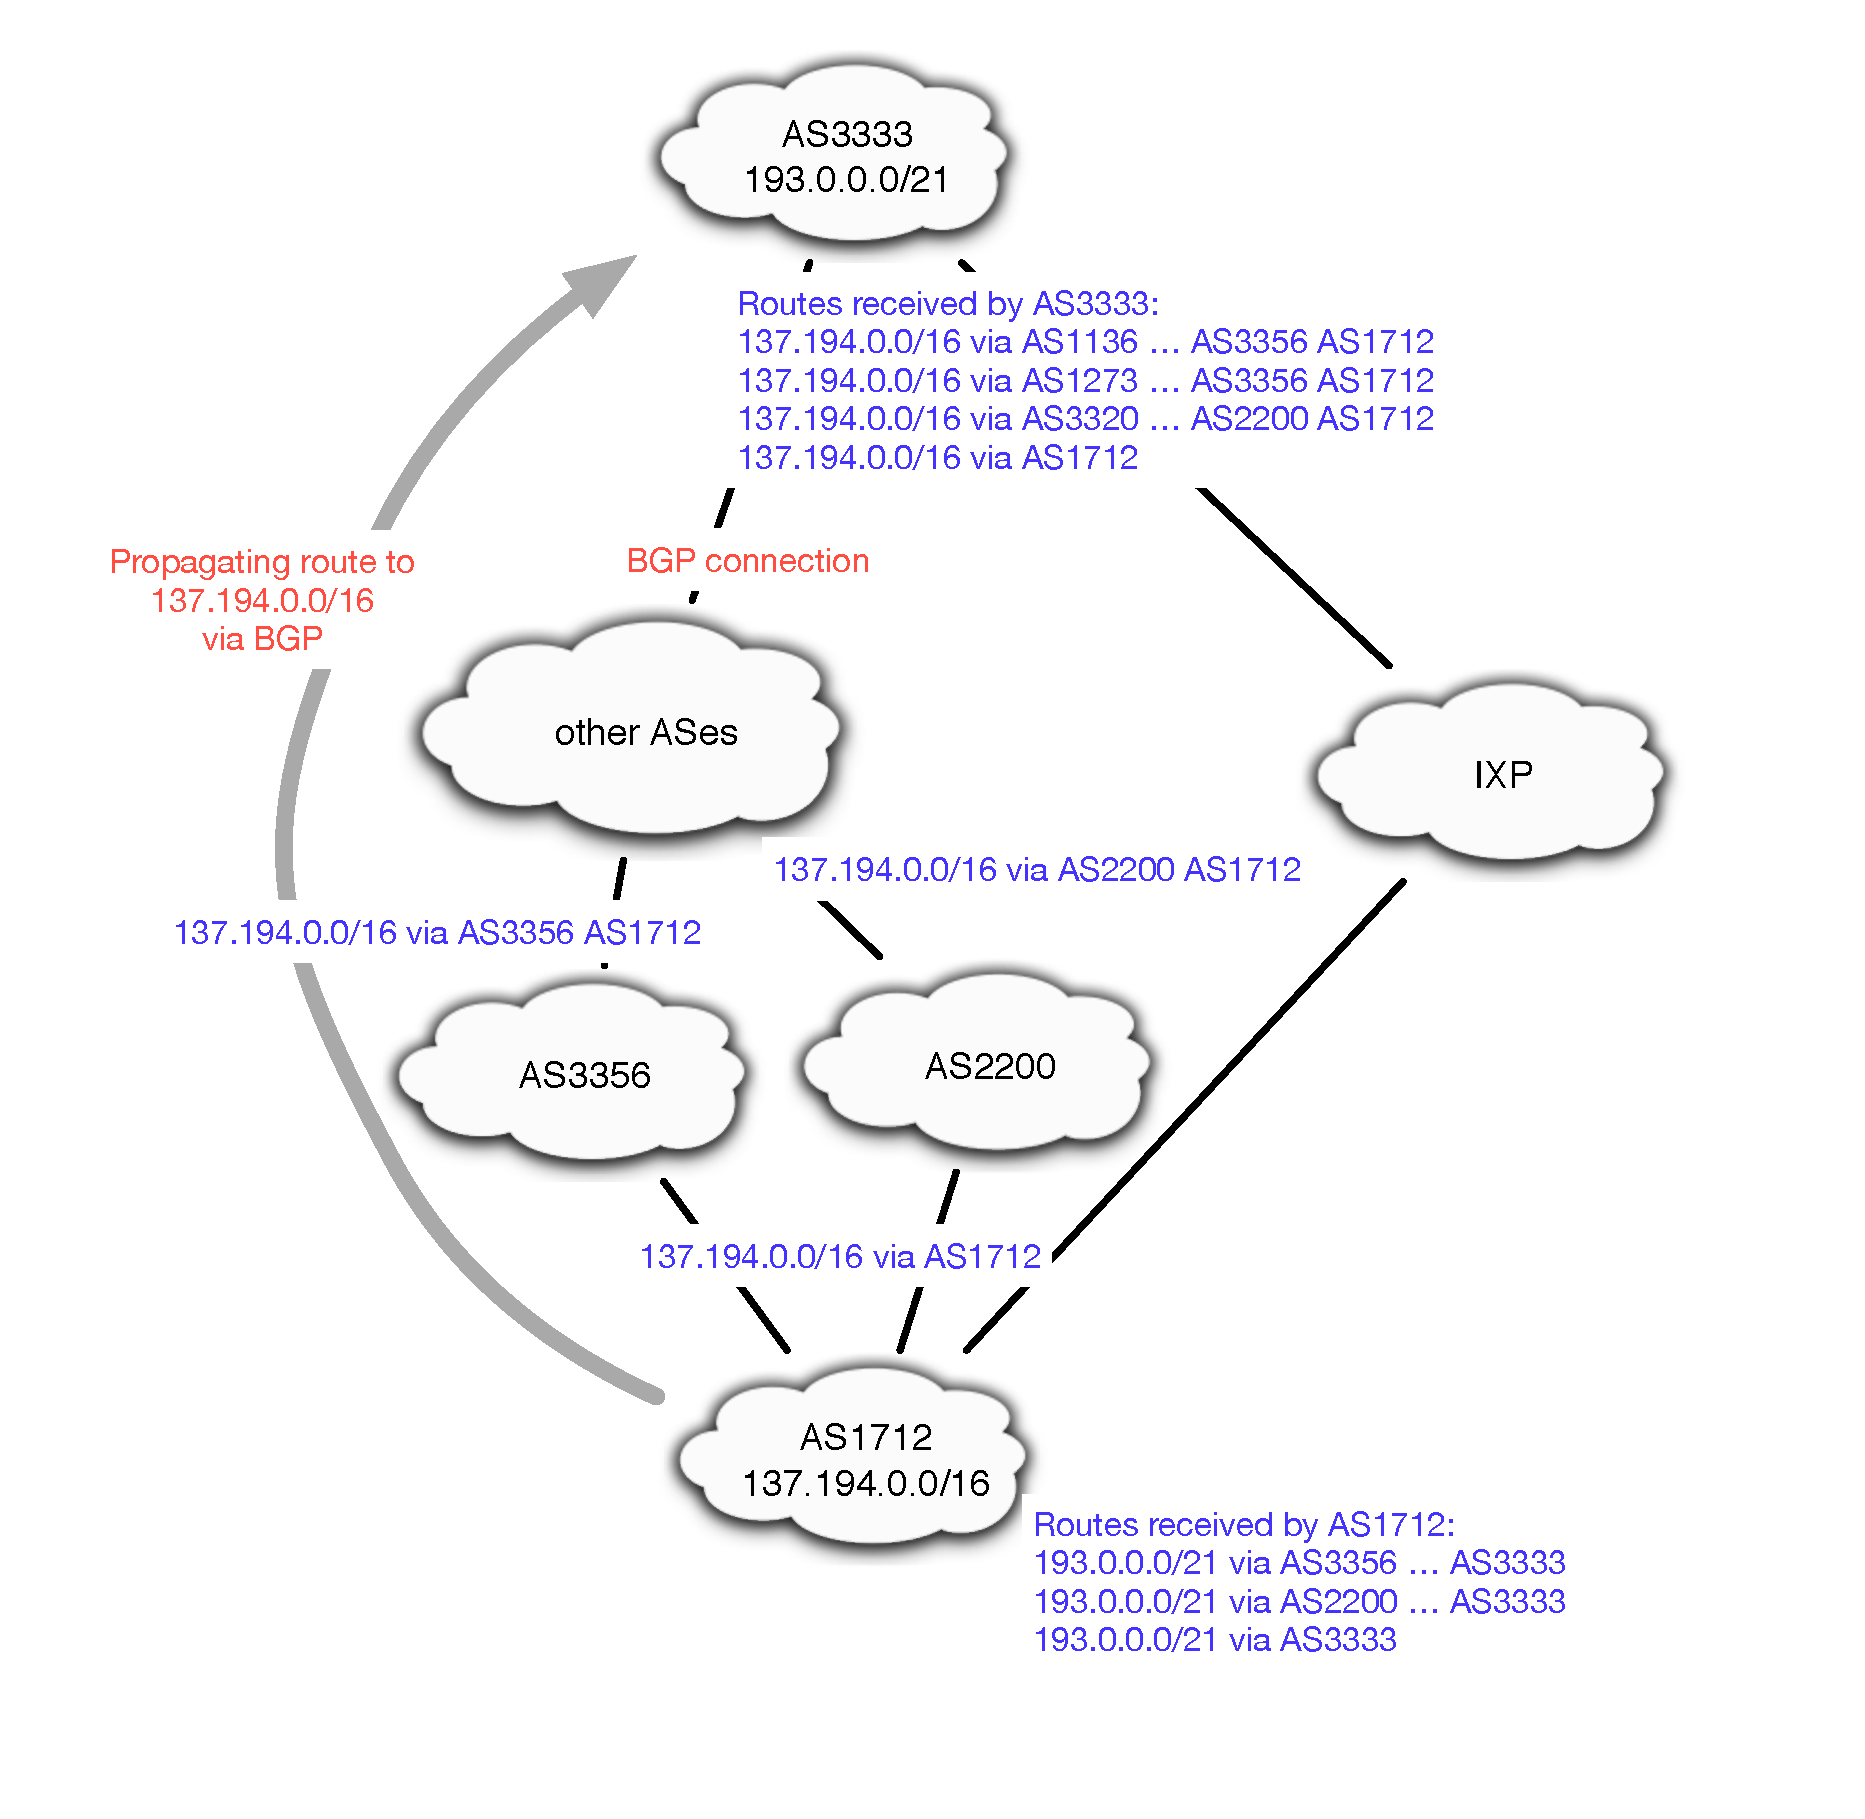
\includegraphics[width=\textwidth]{gfx/chap1/bgp_route_propagation.pdf}
\caption{Interdomain route propagation via \acf{BGP}, an example of \texttt{137.194.0.0/16}\footnote{Networks in this example are fictional}.}
\label{fig:bgp_propa}
\end{figure}

Interconnection of tens of thousands of independently manged networks known as \acf{AS} forms the Internet.
Routing that happens between those ASes is referred to as 
\textit{interdomain routing}.
In order to exchange interdomain routes, each AS uses \acf{BGP}~\cite{bgp4}, a path vector routing protocol, to interface with other ASes.
Fig.~\ref{fig:bgp_propa} illustrates this interaction between ASes. The figure shows how prefix \texttt{137.194.0.0/16} of AS1712 is propagated  to AS3333 via BGP exchanges, so that AS3333 learns the routes on which traffic can be sent to prefix \texttt{137.194.0.0/16}.

There are two types of ASes in above BGP exchanges: \textit{transit provider} and \textit{stub AS}.
Transit provider refers to ASes that offer to route traffic not originated from nor sent to themselves, as a commercial service.
For that purpose, a transit provider announces to its clients all the interdomain routes its learns and to its other BGP neighbors the routes to its clients.
In Fig.~\ref{fig:bgp_propa}, AS3356 and AS2200 are transit providers of AS1712. They help announce the route to prefix \texttt{137.194.0.0/16}
to the rest of the Internet.
On the contrary, a stub AS only cares about sending out its own traffic and becoming reachable to others.
Accordingly, it only announces to its transit providers its own routes. AS1712 is a stub AS in Fig.~\ref{fig:bgp_propa}, as it does not relay interdomain routes for other ASes, and consequently no traffic toward ASes other than itself shall arrive at it.

Besides the transit relationship described above, peering is another type of route and traffic exchange that can happen between two ASes under BGP. Two ASes in peering relationship only exchange with each other their own routes, so that they can directly send traffic to each  without employing a transit provider.
In Fig.~\ref{fig:bgp_propa}, AS1712 and AS3333 directly peer with each other at an \acf{IXP}.
\ac{IXP} is a physical facility that facilitates the establishment of peering relationship. It is transparent to BGP route exchanges.

\section{Interdomain \acf{TE}}
Thanks to transit and/or peering relationship, AS3333 and AS1712 in Fig.~\ref{fig:bgp_propa} may receive multiple routes to a certain destination prefix. Meanwhile, they can as well potentially receive traffic from multiple neighbors.
Such diversity in route brings up two questions: 1) for traffic toward/from a certain prefix, which routes are the best; 2) how to actually steer the traffic on the desired route.
The efforts spared in answering these two questions are referred to as \textit{interdomain \ac{TE}}.

The first question deals with the objective of \ac{TE}. In general, one aims at optimizing the cost and/or performance of transmission.
The second question explores the method of actually routing traffic on the chosen best route. For an AS under BGP routing, its capability in steering traffic is very different on the inbound and the outbound direction. Therefore, the existing practices are summarized respectively.

\subsection{Inbound interdomain TE}
Inbound TE takes care of the incoming traffic distribution on available  links with other ASes.
Since routing with BGP is destination based, it is challenging in precisely steering a part of specific incoming traffic via the desired ingress transit provider. 
It is meaningless defining a best route without effective method to enforce this choice.
Therefore past researches on inbound TE mainly focus on traffic steering method.

By tuning certain BGP attributes when announcing its own route, an AS can potentially influence the BGP route decision process of distant ASes. Some commonly adopted practices are: selective announcement, more specific announcement, AS path prepending, setting \acf{MED} and employing community attribute supported by certain transit provider~\cite{Wang2008}.

These approaches are not perfect. Selective announcement introduces reachability risks, while more specific announcement gives rise to \acf{RIB} inflation. AS path prepending is as well shown to be not effective in avoiding using a specific transit provider due to the fact that is very hard to predict the BGP route choice of distance ASes~\cite{Quoitin2004a}. BGP community~\cite{Donnet2008, Shao2015} and later on redistributed communities~c\ite{Quoitin2002} allow finer grained operations with better certainty. However, it requires the support from transit providers. 

Some other approaches dictates the incoming path by changing the traffic source address through encapsulation~\cite{Liu2008} or \acf{NAT}~\cite{Sun2015}. However, traffic with source address outside the prefixes announced to it BGP neighbors can be filtered for security considerations, especially for ASes meant to use IP addresses assigned by its transit provider~\cite{filtering}.
\acf{LISP} pushes such approach to a revolutionary level by introducing a separate addressing space in the core of Internet for TE purposes~\cite{lisp}. Studies show fine-grained and dynamic inbound optimization is feasible with fare cost under \ac{LISP}~\cite{Iannone2007, saucez2011mechanisms, quoitin2007evaluating}.



\subsection{Outbound interdomain TE}
How to select the best route for each destination prefix and send out the traffic correspondingly is known as outbound TE. 
An AS has total control over the egress route employed in reaching each destination prefix. Common practice is to tune \textit{local preference} BGP attributes~\cite{Wang2008}. 
Therefor the challenge is rather on the composition of best routes in terms of cost and performance.

The cost of interdomain transmission depends on the the amount of traffic exchanged on links purchased from transit providers~\cite{drpeering-95th}.
Meanwhile, whether these transit links are congested impacts as well the transmission performance.
Hence, outbound TE resolves in routing appropriate amount of traffic on each available transit links to lower the transit cost while not surpassing the capacity of each link (especially the cheapest one).
\cite{Goldenberg2004} formulated this quest as a minimum-cost multi-commodity flow problem when avoiding transit link congestion under transit cost constraints.
\cite{Uhlig2004b} fulfills the same goal while minimizing the number of route changes required.
\cite{Zhu2014} avoids congestion on transit links by including border router queue length in route decision.

Indeed, it is unwise to allow congestion on transit links that can be directly monitored.
However, there are many other factors that may as well put transmission performance in danger.
The minimum delay of Internet transmission toward a destination is dominated by the physical length traversed. 
On top of that, transient events like congestion can happened in the middle of the Internet~\cite{Akella2003, Luckie2014}.
In order to first learn the presence of these issues and then optimize the routing against these events, end-to-end delay measurement is indispensable in cumulatively reflecting the delay contribution from each element of the forwarding chain, including the local link to transit providers.

\subsection{\ac{SDN} and interdomain TE}
Recently, \acf{SDN} contributes as well to interdomain TE. The common part of these ideas is to delegate the TE decision and execution of an AS to a third party, where route decisions can be performed in a centralized manner in accordance to \ac{SDN} design philosophy. It is advocated that the interdomain TE can hence be done in a more cooperative way, and is for the good of larger optimality. Moreover, conflicts in TE policies can as well be solved in a centralized manner.
\cite{Kotronis2012} advances that such ASes clusters under same TE service provider can be formed in an gradual way and eventual drives the evolution of the interdomain routing.
SDX~\cite{Gupta2014} focuses on the application of \ac{SDN} in a more specific network environment, \ac{IXP}, where members by nature forms a cluster of ASes that exchange their routing information along with their TE polices within one centrally managed facility. Application specific peering, e.g. only peer for the exchange of video traffic, is made possible under this framework.

\subsection{Scope of this thesis}
We stage the works of this thesis under BGP, while fully realizing \ac{LISP}, \ac{SDN} and etc. are promising directions to pursuit.
It is because for BGP is still going to be the \textit{de facto} routing protocol of the Internet in the foreseeable future, for the deployment of new routing mechanism must be incremental.
Till then,  BGP is what a majority of ASes has to live with and there are still spaces for improvements.
We focus on outbound TE in this thesis, as inbound TE has been shown to be inherently difficult with BGP.
We target stub ASes (potentially multi-homed), since dynamic route re-selection in those networks will not cast Internet-wide BGP route convergence issues.
Meantime, \acf{CP}, \acf{HP} and \acf{ISP}, being major network types among stub ASes, are those who needs most outbound TE.
Finally, we assume improving transmission performance is major motivation for outbound TE in these stub ASes.
Continuously decreasing transit price~\cite{transitprice, drpeering} and high \ac{IXP} growth rate worldwide~\cite{pchixp} indicate that routing traffic throughout the Internet now faces less monetary constraints but rather encounters a performance challenge that could be potentially lifted with geographical and topological connection diversity~\cite{Chiu2015}.

\section{Measurement-based TE and motivations}

BGP itself is one big obstacle in the pursuit for better transmission performance, as its route decision mechanism is unaware of the performance characteristics of candidate paths~\cite{Yannuzzi2005}.
However, not all interdomain routes offer the same transmission performance. \cite{Akella2003} points out that bandwidth bottleneck can be within certain \acp{ISP} or on the links between \acp{ISP}, suggesting that the choice of transit provide is not without impact on transmission performance.
Further, \cite{Akella2003a} quantified the potential performance gain an AS could achieve with multi-homing.
\cite{Akella2004} advocates that this gain is not far away from that of overlay networking.

In order to actually realize this performance gain, a system that dynamically selects for each destination the best performing route according to real-time measurements is required, i.e. \textit{measurement-based TE}.
\cite{Akella2008} presents a demo implementation of such a system that makes outbound TE decision based on end-to-end delay measurements. Only 100 destinations are emulated in this work, far less than the actually number a stub AS might face on a daily base. Best route is chosen based on the \acf{EWMA} of past end-to-end delay measurements. It turned out that when no history record is considered, best overall transmission performance is achieved. However, considering the noisy nature of RTT measurements, such a simplistic approach can lead to overwhelmingly frequent path changes. Moreover, treating the Internet as a blackbox for delay measurements does not provide useful and necessary visibility to the stub AS regarding the actual network events that cause significant performance degradation and hence justify the TE decisions made. 


Bearing the above in mind, we aim to address some of the measurement related problems in building a interdomain TE platform that works in the real world.


\section{Road map}
\subsection{Building blocks of measurement-based TE}

\begin{figure}[!htb]
\centering
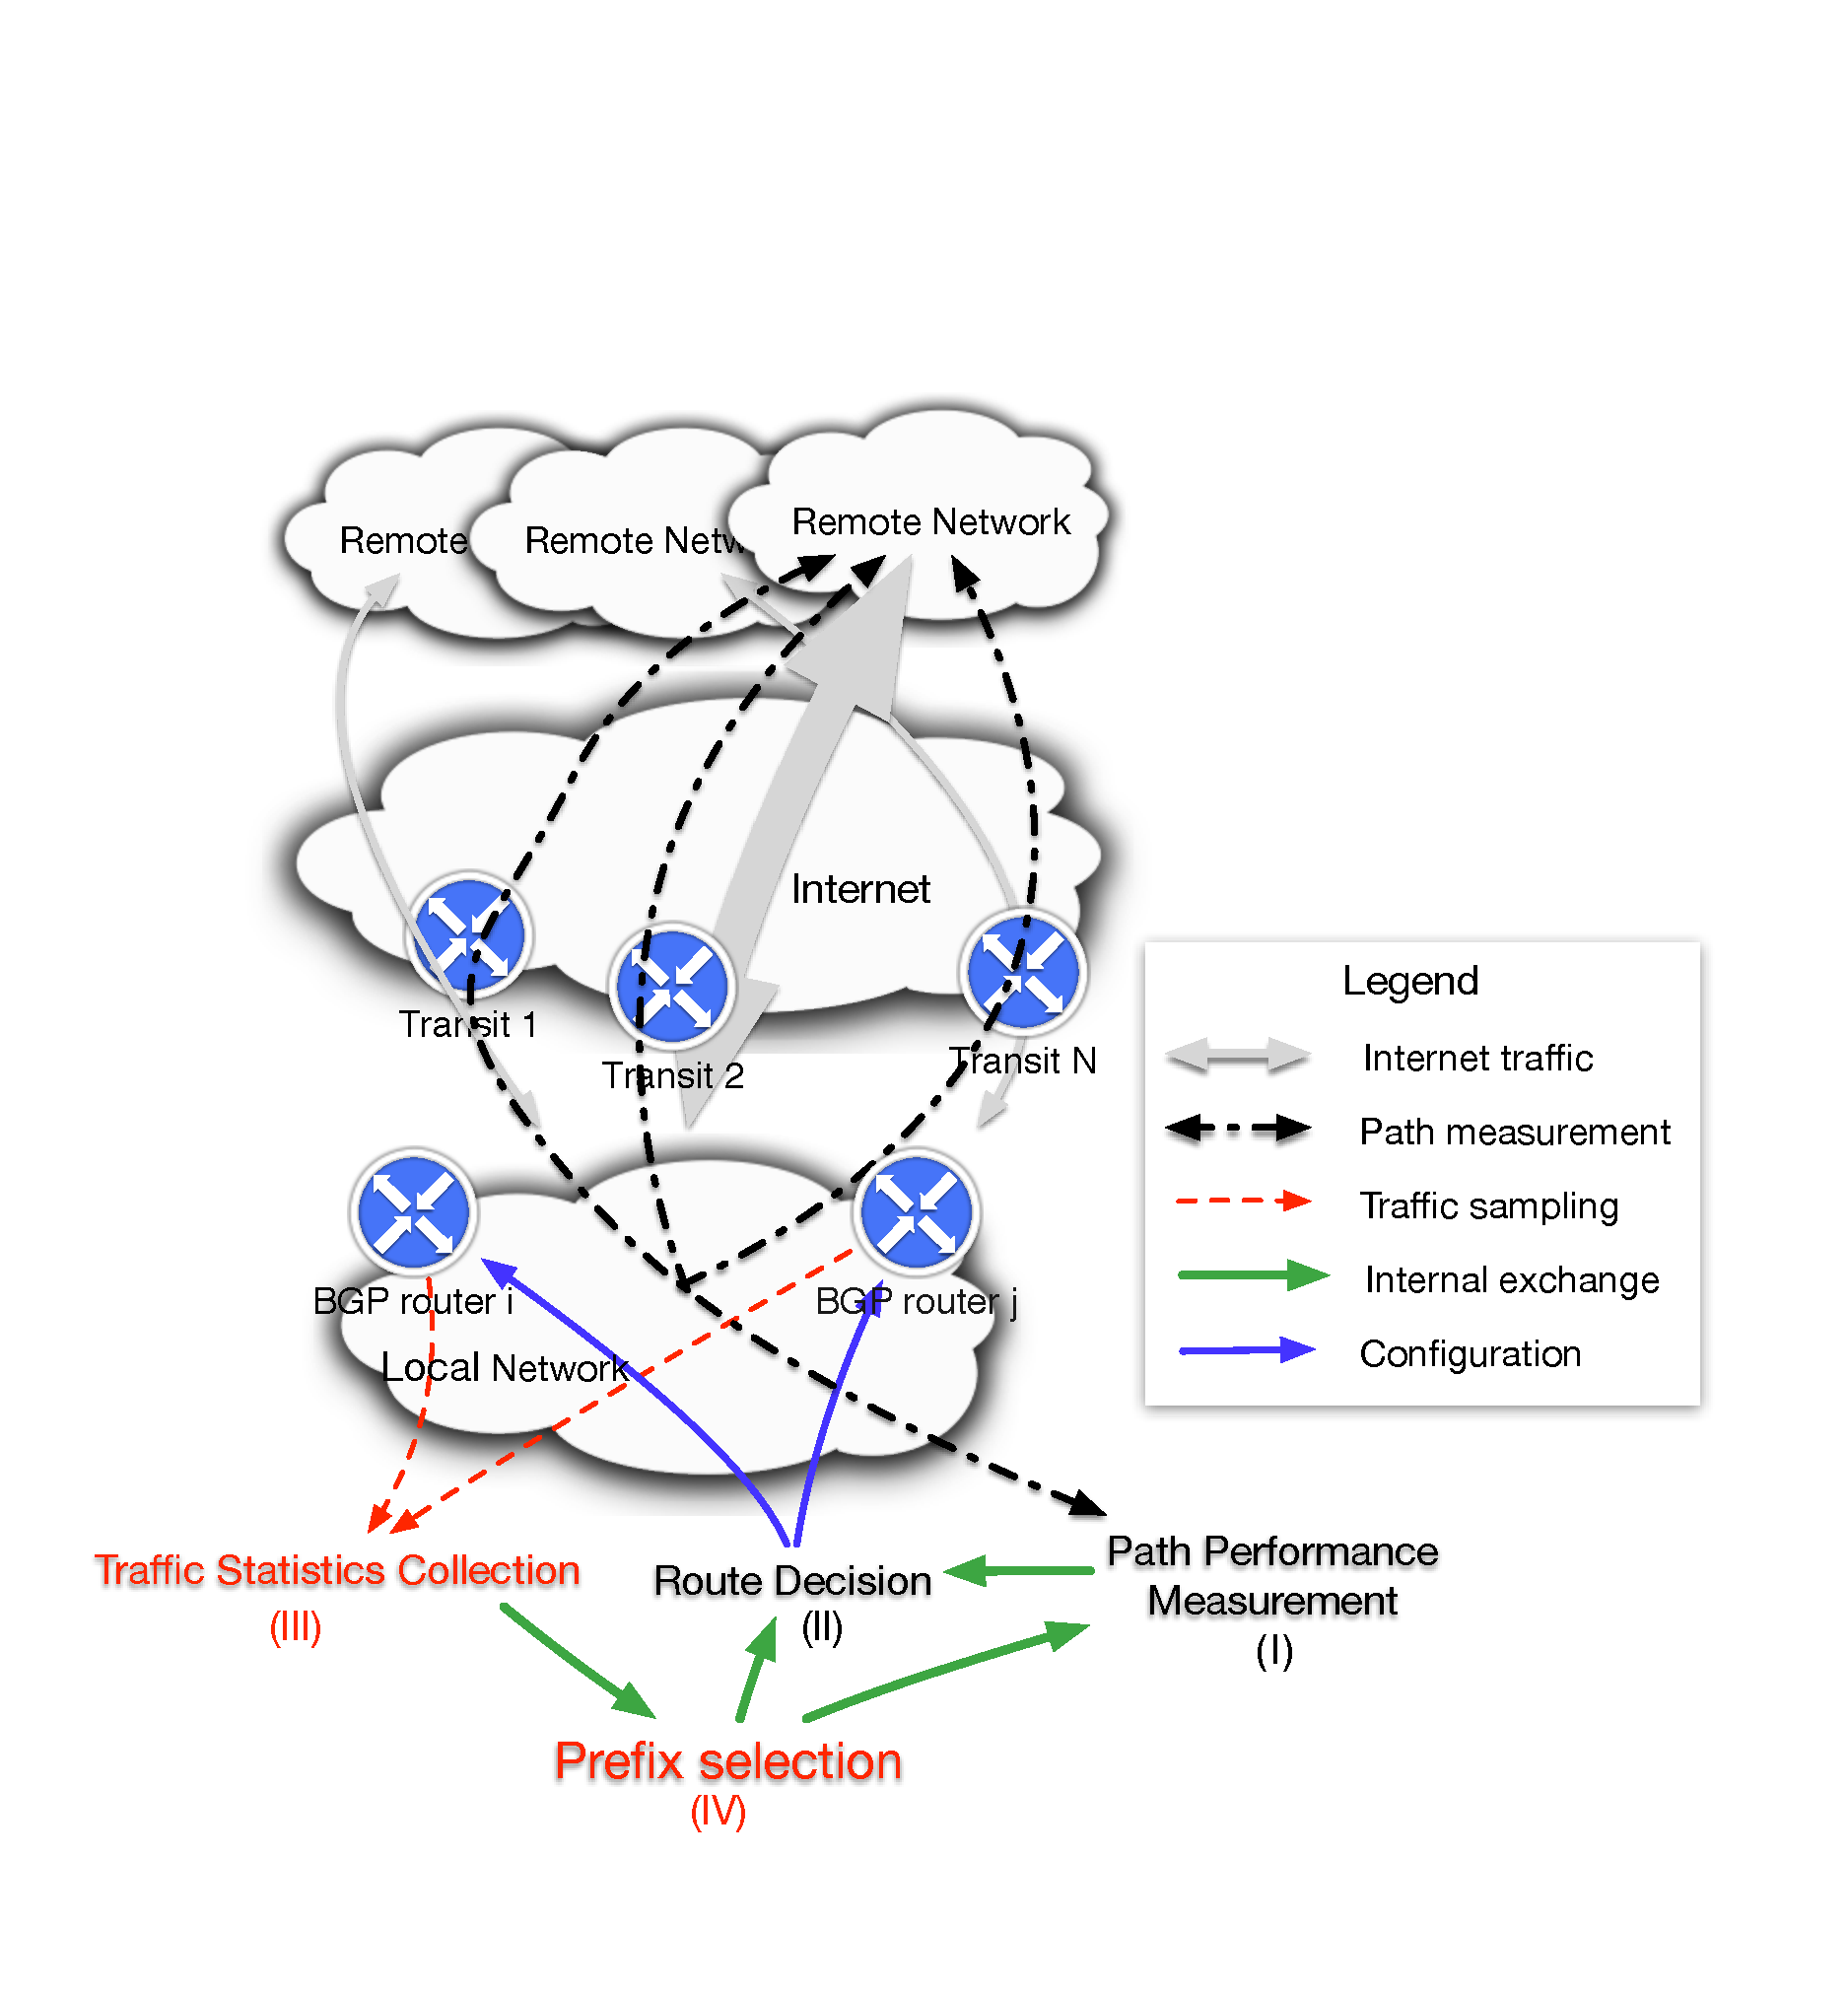
\includegraphics[width=\textwidth]{gfx/chap1/archi.pdf}
\caption{Building blocks of measurement-based inter-domain TE system.}
\label{fig:archi}
\end{figure}

A measurement-based interdomain TE platform has two essential building blocks illustrated in black in Fig.~\ref{fig:archi}: (i) path performance measurement and (ii) route decision.
Since each destination prefix may have multiple available routes, the platform has to measure in a repeated manner the end-to-end performance over all these routes. 
For each destination prefix, a couple of hosts with known open ports, e.g. 80, 443, are discovered and used as probing destination in delay measurements.
Once fed with performance metrics, route decision engine dictates,  taking into account other constraints such as routing policies, for each destination which is the best route at a certain moment and imposes it on BGP border routers.

\subsection{Prefix selection: focus on most important destinations}
However, a scalability issue presents in the above design as a stub AS can exchange with up to 100k destination prefixes.
Continuous performance monitoring to all of these destinations over all available paths is going to be prohibitively costly.
\cite{Feamster2003} already realizes this issue and proposes to focus on popular destinations.
However, no solution is given.
In Chapter~\ref{sec:pref_selec} we tackle the selection of prefixes associated with important traffic volume by studying their temporal dynamism at different time resolutions. Two additional building blocks (in red) are hence added to Fig.~\ref{fig:archi}.

\subsection{RTT measurements with RIPE Atlas}
Studies in Chapter~\ref{sec:pref_selec} solely base on the measurement data collected by BORDER 6 proprietary TE platform from client networks. Such working trace from real networks increases the credibility of our observation. However, it brings as well reproducibility concerns.
In Chapter~\ref{sec:ripe_atlas}, we first justify our choice of using RIPE Atlas~\cite{atlas} as our source of path and delay measurements for later researches.
We then discuss a data quality issue stemmed from the measurement platform.

With the openly accessible measurements from RIPE Atlas, we investigated another data quality issue, which is specific to the context of interdomain TE this time. When measuring a same AS path with multiple different \acf{RTT} measurements toward different hosts in the destination prefix, what will these RTT time series look like? Will they have similar characters? If not, how can we pick out the ones fit best for our TE uses? We employ clustering methods to reveal the inherent structure of a such set of RTT time series.

During the above study, we notice an interesting phenomenon where several RTT time series have a similar shape at the same moment. Such synchronized RTT change is exclusive to this small group of measurements.
We thus find it promising to infer the actually location of shared RTT changes by grouping RTT time series of similar shape. To that end, we study the application of time series clustering methods to RTT measurements and discuss its limitations.

\subsection{Change detection for RTT measurements}
The case of RTT time series with similar shape leads to further studies in Chapter~\ref{sec:cpt_rtt} and \ref{sec:infer}. Chapter~\ref{sec:cpt_rtt} studies the application of changepoint detection methods on RTT measurements. These methods detecting significant changes in time series is regarded as an expressive way to simply the representation of RTT measurements. Meantime, we realize that the detected moments of change can serve as an informative and robust trigger for route re-selection.
Since RTT measurements are rarely covered in previous change detection studies. To quantify the detection performance with RTT measurements, we build an evaluation framework and benchmark several candidate methods.
The temporal correlation between RTT changes and routing events are as well studied and illustrated.

\subsection{Inferring the location of RTT changes}
With simplified data representation enabled by changepoint detection, we study the method inferring the location of detected RTT changes.
Knowing the location of RTT changes are of significance in measurement-based interdomain TE,  especially for a non-negligible part of destinations that we are not able to measure. Knowing the location causing RTT change can thus help making proper route decisions to avoid certain problematic paths.

To that end, we first group RTT time series undergoing same RTT changes with the help of change detection.
Then inference logic are developed to attribute RTT change cause to ASes and links basing on two simple and intuitive assumptions.
Visualization tools are as well made to illustrate the inference logic and the inferred location of change on an AS-level topology learnt from measurements.
